\documentclass[twoside,numberorder]{csbachelor}

%==============================================================
%==============================================================

\usepackage{url}
\usepackage{subfigure}

% 张海:其他引用
\usepackage{hyperref}
\usepackage{pdfpages}

% 一些全局工具的定义
\DeclareMathOperator*{\argmin}{arg\,min}
\DeclareMathOperator*{\argmax}{arg\,max}

%==============================================================
%==============================================================
\usepackage[square,numbers,sectionbib]{natbib}
\usepackage{chapterbib}
\begin{document}

\pagestyle{empty}

%==============================================================
%==============================================================

  % 论文题目:{中文}{英文}
  \zjutitle{标题}
           {Title}
  % 作者:{中文姓名}{英文}{学号}
  \zjuauthor{姓名}{Name}{313XXXXXXXX}
  % 指导教师:{导师中文名}{导师英文名}
  \zjumentor{导师姓名}{Supervisor name}
  % 个人信息:{年级}{专业名称}
  \zjuinfo{2013级}{计算机科学与技术}
  % 学院信息:{学院中文}{学院英文}
  \zjucollege{计算机科学与技术学院}{College of Computer Science and Technology}
  % 日期:{Submitted Date}
  %\zjudate{2017-03-29}

%==============================================================

  \thispagestyle{empty}

{
\setlength{\parindent}{0em}
\renewcommand{\baselinestretch}{2}

\vspace*{-7mm}

\begin{center}
  \includegraphics[width=108mm]{data/cover/xiaoming}
\end{center}

\vspace{-1mm}

{
\renewcommand{\baselinestretch}{1.8}
\heiti\xiaoyi\bfseries
\centering
本~~科~~生~~毕~~业~~论~~文~~(设计) \\
文献综述和开题报告 \par
}

\vspace{4em}

\begin{center}
  \includegraphics[width=35mm]{data/cover/xiaobiao}
\end{center}

\vspace{3em}

{
\renewcommand{\baselinestretch}{1.65}
\stfangsong\sanhao\bfseries
\centering
% 题目 \; \underline{\makebox[16em]{\zjutitlec}} \\
学生姓名 \;\;\; \underline{\makebox[12em]{\zjuauthornamec}} \vspace{1em}  \\
学生学号 \;\;\; \underline{\makebox[12em]{\zjuauthorid}} \vspace{1em} \\
% 学号 \; \underline{\makebox[16em]{\zjuauthorid}} \\
指导教师 \;\;\;\;\;\; \underline{\makebox[12em]{\zjumentorc}} \vspace{1em}  \\
年级与专业 \;\;\; \underline{\makebox[12em]{\zjugrade~~\zjumajor}} \vspace{1em}  \\
所在学院 \;\;\;\;\;\; \underline{\makebox[12em]{\zjucollegec}} \par
}
}

\ifthenelse{\equal{\zjuside}{T}}{\newpage\mbox{}\thispagestyle{empty}}{}


  \newpage

\thispagestyle{empty}

% \vspace*{0.0em}

{
\setlength{\parindent}{0em}
\renewcommand{\baselinestretch}{2}
\stfangsong\sihao\bfseries

一、 \; 题目: \; \zjutitlec

\vspace{0.5em}

二、 \; 指导教师对文献综述和开题报告的具体要求:

% \begin{enumerate}
%     \item 开题报告需内容详实,工作量分配合理,格式正确。对项目中各项流程有基本的规划,并且提出初步的技术方案,对其中所需的各项技术有一定的了解和认识。其它参照学院和学校相关规定。
%     \item 外文翻译格式正确,翻译内容与原文无出入且易于理解。其它参照学院和学校相关规定。
%     \item 文献综述涵盖论文最重要的相关文献,对现有方法有良好的分类分析,特别是对计划中比对的方法有较明确的分析和阐述。其他参照学院和学校的相关规定。
% \end{enumerate}

% \vspace{8cm}
\vspace*{\fill}
}

{
\stfangsong\xiaosi\bfseries
\begin{flushright}
  指导教师(签名) \; \uwave{\hspace{5em}}  \hspace*{3em}  \\
  \vspace{1em}
  年 \qquad 月 \qquad 日 \hspace*{1em} \hspace*{3em}
\end{flushright}

\vspace{0.5cm}
}

\ifthenelse{\equal{\zjuside}{T}}{\newpage\mbox{}\thispagestyle{empty}}{}


  \thispagestyle{empty}

{
  \setlength{\parindent}{0em}
  \renewcommand{\baselinestretch}{2}

  {
    \stfangsong\sanhao\bfseries
    \centering
    毕业设计开题报告、外文翻译和文献综述的考核 \par
  }

  {
    \songti\sihao\bfseries
    导师对开题报告、外文翻译和文献综述的评语及成绩评定:

    \vspace{8em}

    {
      \renewcommand{\baselinestretch}{1}

      \begin{flushright}

        \begin{tabular}{|c|c|c|c|c|}
          \hline
          成绩比例 & \parbox[c]{3.6em}{\xiaosi 开题报告 \\ 占(20\%) \vspace{0.25em}} & \parbox[c]{3.6em}{\xiaosi 外文翻译 \\ 占(10\%) \vspace{0.25em}} & \parbox[c]{3.6em}{\xiaosi 文献综述 \\ 占(10\%) \vspace{0.25em}}\\
          \hline
          分值 & & & \\
          \hline
        \end{tabular}

        \vspace{2em}

        {
          \songti\xiaosi\bfseries
          导师签名 \; \underline{\hspace{6em}} \hspace*{3em} \\
          年 \qquad 月 \qquad 日 \hspace*{3em} \par
        }
      \end{flushright}
    }
  }

  \vspace{1em}

  {
    \songti\sihao\bfseries
    学院盲审专家对开题报告、外文翻译和文献综述的评语及成绩评定:

    \vspace{12em}

    {
      \renewcommand{\baselinestretch}{1}

      \begin{flushright}

        \begin{tabular}{|c|c|c|c|c|}
          \hline
          成绩比例 & \parbox[c]{3.6em}{\xiaosi 开题报告 \\ 占(20\%) \vspace{0.25em}} & \parbox[c]{3.6em}{\xiaosi 外文翻译 \\ 占(10\%) \vspace{0.25em}} & \parbox[c]{3.6em}{\xiaosi 文献综述 \\ 占(10\%) \vspace{0.25em}}\\
          \hline
          分值 & & & \\
          \hline
        \end{tabular}

        \vspace{2em}

        {
          \songti\xiaosi\bfseries
          开题报告审核负责人(签名/签章) \; \underline{\hspace{6em}} \hspace*{3em} \par
        }
      \end{flushright}
    }
  }

  \ifthenelse{\equal{\zjuside}{T}}{\newpage\mbox{}\thispagestyle{empty}}{}
}


  \tableofcontents
  \thispagestyle{toc}
  %\chaptermark{目录}

  \mainmatter

  {
    \pagestyle{kaitibaogao}
    \makeatletter
      \let\ps@plain\ps@kaitibaogao
    \makeatother
    \chapter{开题报告}

\section{问题提出的背景}
cite something~\cite{article1}
\subsection{背景介绍}

\subsection{本研究的意义和目的}

\section{论文的主要内容和技术路线}

\subsection{主要研究内容}

\subsection{技术路线}

\subsection{可行性分析}

\section{研究计划进度安排及预期目标}

\subsection{进度安排}

\subsection{预期目标}

\bibliographystyle{data/gbt7714-2005}
{
\renewcommand{\bibsection}{\section{\bibname}}
\bibliography{data/cite}
}

% 按文章长度需要启用
\ifthenelse{\equal{\zjuside}{T}}{\newpage\mbox{}\thispagestyle{empty}}{}

  }

  {
    \pagestyle{waiwenfanyi}
    \makeatletter
      \let\ps@plain\ps@waiwenfanyi
    \makeatother
    \setcounter{page}{1}

    \renewcommand{\addcontentsline}[3]{}

    {
\renewcommand{\baselinestretch}{1.25}\selectfont

{
  \titleformat{\chapter}[block]{\erhao\songti\bfseries\filcenter}{}{0em}{}{}
  \chapter{本科毕业论文外文翻译}
}

{
  \setlength{\parindent}{0em}

  文献原文:

  A. Bravo, C. Delta. How to translate a sample paper. 2017. \par
}

\vspace{2em}

{
  \renewcommand{\cleardoublepage}{}
  \renewcommand{\clearpage}{}
  \titleformat{\chapter}[block]{\sanhao\songti\bfseries\filcenter}{}{0em}{}{}
  \chapter*{外文翻译标题}
}

\section*{摘要}

\section{前言}

\begin{figure}[!htbp]
\centering
\includegraphics[width=\linewidth,keepaspectratio]{data/waiwenfanyi/placeholder.png}
\caption{Placeholder}
\label{figure:placeholder}
\end{figure}

图~\ref{figure:placeholder}

手动引用~1 {[}1{]}

\section*{参考文献}

\begin{itemize}
\item [{[}1{]}] A. Baker, C. Dog. How to make a sample reference. 1938.
\end{itemize}
}

% 按文章长度需要启用
%\ifthenelse{\equal{\zjuside}{T}}{\newpage\mbox{}\thispagestyle{empty}}{}

  }

%  \backmatter

  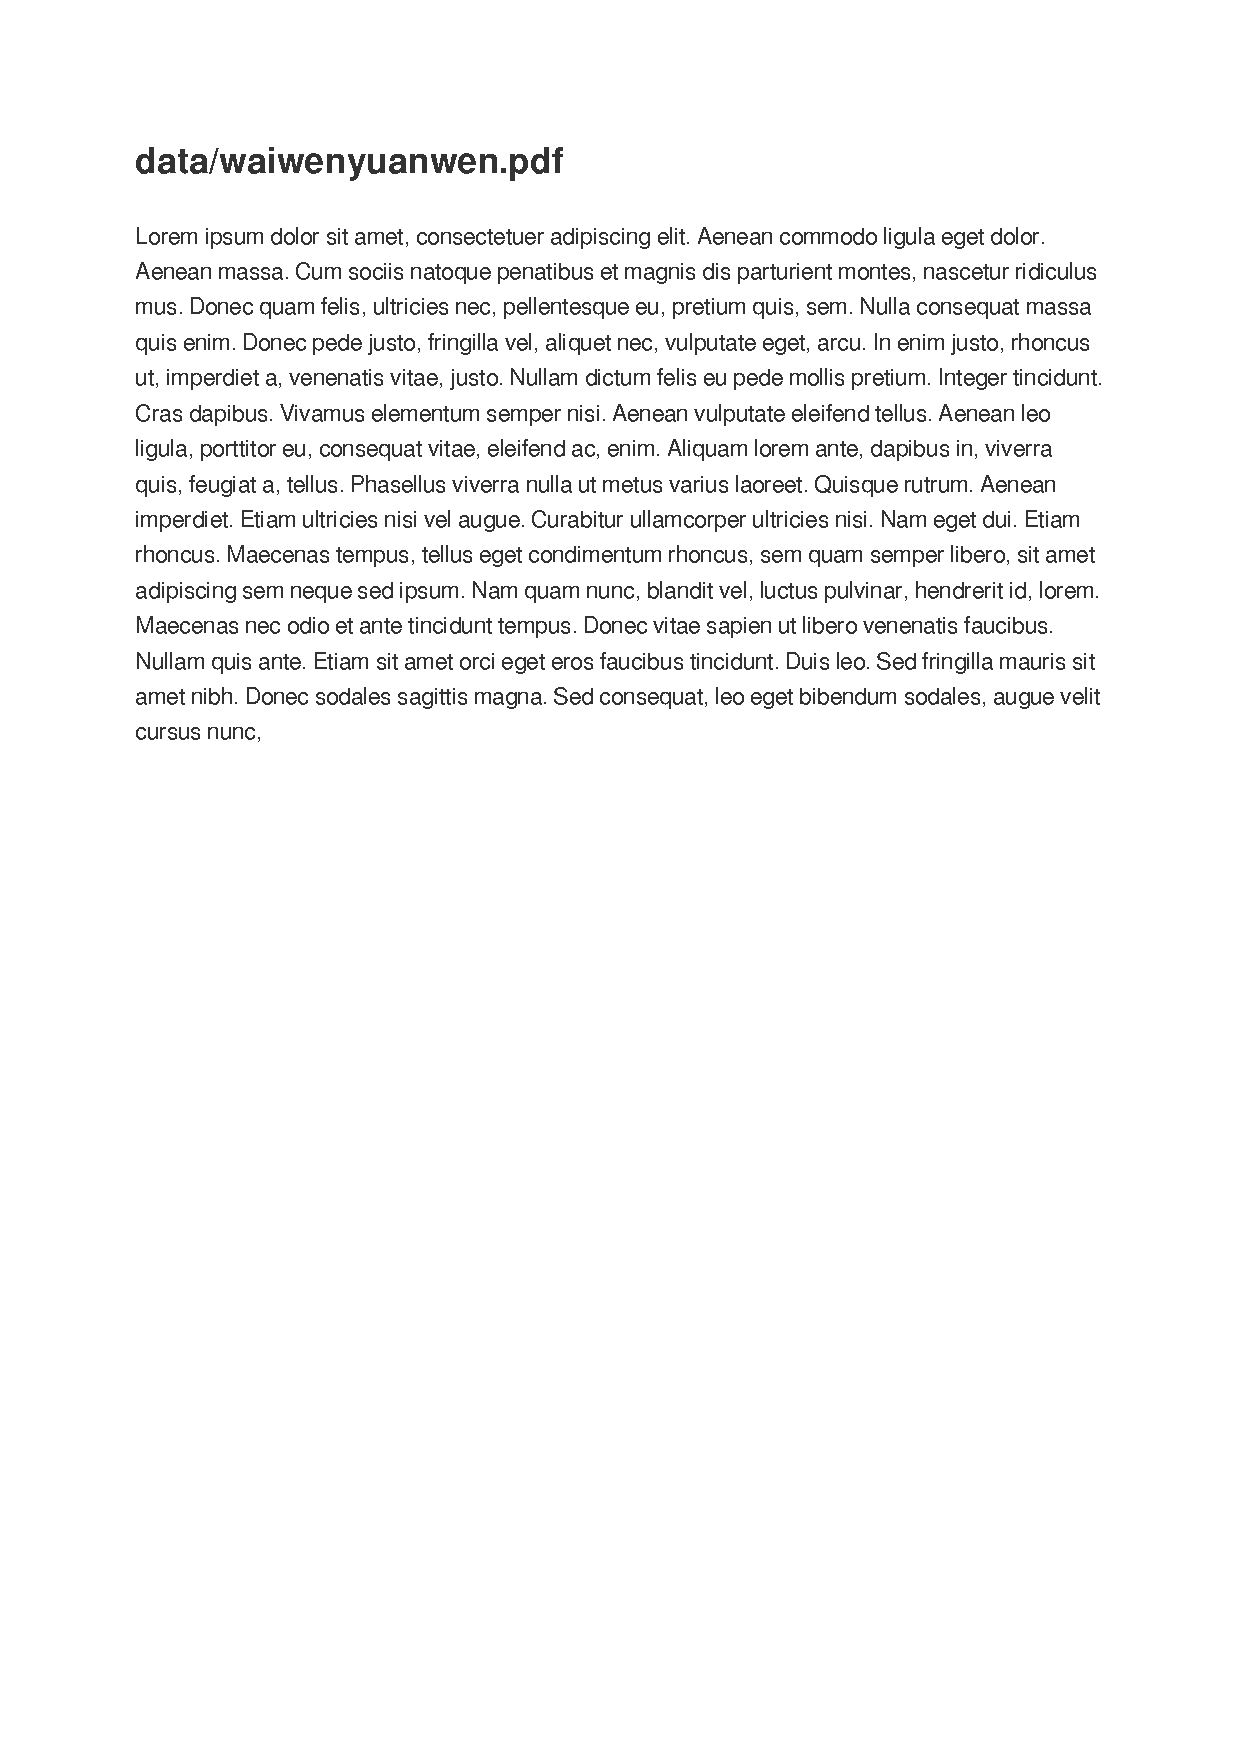
\includepdf[pages=-]{data/waiwenyuanwen.pdf}

  {
    \pagestyle{wenxianzongshu}
    \makeatletter
      \let\ps@plain\ps@wenxianzongshu
    \makeatother
    \setcounter{page}{1}

    \renewcommand{\addcontentsline}[3]{}

    \chapter{文献综述}

\section{背景介绍}
cite something~\cite{article1}
\section{国内外研究现状}

\subsection{研究方向及发展}

\subsection{存在问题}

\section{研究展望}

\bibliographystyle{data/gbt7714-2005}
{
\renewcommand{\bibsection}{\section{\bibname}}
\bibliography{data/cite}
}


% 按文章长度需要启用
%\ifthenelse{\equal{\zjuside}{T}}{\newpage\mbox{}\thispagestyle{empty}}{}

  }


\end{document}
